\documentclass[letterpaper,10pt]{article}

%\setlength{\parindent}{0in}
%\usepackage{fullpage} 
\usepackage{amsmath}
\usepackage{amssymb}
\usepackage{enumerate}
\usepackage{graphicx}
\usepackage{color}
\usepackage[table]{xcolor}
\usepackage{dcolumn}
\oddsidemargin 0.0in
\textwidth 6.5in
\newcolumntype{.}{D{.}{.}{-1}}
\newcommand*{\myalign}[2]{\multicolumn{1}{#1}{#2}}

% Project Assignment 3 (Module 7):  (15 points � 12 points for the assignment 
% and 3 points for each individual role playing DB submission)
% Project Assignment 3 Cost is a team event and is due 2/24/12. Please see the 
% Project area in Sakai for more guidance.
% Determine the Life Cycle Cost (LCC) and Total Ownership Cost (TOC) of the 
% prototype robot variants, using the robot configurations, cost data, and 
% estimation spreadsheet provided. The SMETAL LCC Estimate cost equation 
% provided is the cost for one robot.
% a) Estimate the discounted LCC and TOC for a ten (10) year period, discounted 
% at a rate of 6%. The cost data and spreadsheet model provided does not include 
% aspects related to TOC.
% b) Make some reasonable assumptions about the TOC.
% c) Create a TOC spreadsheet model to develop the TOC estimate for each 
% variant.
% d) Create a LCC profile for each variant in accordance with B&F chapter 17.
% e) Summarize and present the results of your analysis.
% Remember to complete your RPG Role Evaluation on the Discussion Board 
% also!

\title{Project 3 \\ \Large Team CLEAR \\ \normalsize (\textcolor{red}{C}onvoy \textcolor{red}{L}evel \textcolor{red}{E}xplosive \textcolor{red}{A}mmunition \textcolor{red}{R}emoval)}
\author{Christian Aall: Testing \& Evaluation \\ 
	Steve Mazza: Team Lead \\ 
	Michael Oexmann: Analyst \\ 
	Elizabeth Swisher: Lead Systems Engineer}
	
\date{February 24, 2012}

\begin{document}
\maketitle
\tableofcontents
\listoftables
\listoffigures

\pagebreak
In this report, CLEAR attempts to provide a TOC and LCC assessment for the SMETAL-V system. An initial cost assessment of a system, coupled with a prototype variant down selection based on parameter performance, allows a decision maker to make a superficial decision on which prototype variant to transition into production. To ensure the customer receives the most suitable variant, at the best price for the given deployment scenario, further analysis must be performed. By evaluating and measuring all cost contributors, both direct and indirect, to the system's predicted or required life-span one may gain insight into additional, perhaps even hidden costs associated with maintaining system mission readiness. Through the use of software-based data analysis tools and a graphical presentation of the results, CLEAR believes that this report will serve as a comprehensive means of down selecting system variants based on TOC incurred by the customer during the deployment of the SMETAL-V system.

\section{Discounted LCC \& TOC}
In order to determine the Life Cycle Cost (LCC) and Total Ownership Cost (TOC), over a ten year period, of the prototype robot variants ($A$, $B$, and $C$), cost estimation spreadsheets shown in Appendix \ref{sec:workbooks} were utilized. Although another variant (variant $D$) has been developed, LCC and TOC have not been calculated as this variant has not yet been tested. These spreadsheets take into consideration, a discount of 6\%, learning rate of approximately 0.92 and assume the production of 10 units per year. A comparison of LCC and TOC estimates can be seen in Table \ref{tab:requirementA} on page \pageref{tab:requirementA}.

\begin{table}[h!tbp]
	\begin{center}
		\begin{tabular}{l...}
			\hline
			& \myalign{c}{\textbf{Variant A}} & \myalign{c}{\textbf{Variant B}} & \myalign{c}{\textbf{Variant C}} \\
			\hline\hline
			LCC, 10 yr, 6\% discount &	\$7,224,937.04 &	\$11,960,055.10 &	\$7,318,145.56 \\
			TOC, 10 yr, 6\% discount &	\$8,329,937.04 &	\$13,065,055.10 &	\$8,423,145.56 \\
			\hline
		\end{tabular}
	\end{center}
	\caption{Comparison of LCC and TOC estimates}
	\label{tab:requirementA}
\end{table}

These results indicate that variant $A$ is the overall least expensive option both in LCC and TOC over 10 years.

\section{Assumptions}
We were presented with certain \emph{givens} from which we made some reasonable assumptions.  Those are documented below and reflect the previous analysis as well as our collective domain knowledge, research, and experience.

\begin{itemize}
\item Given 
	\begin{itemize}
		\item It is given that training cost is \$10,000 per initial operator.
		\item It is given that training cost is a onetime cost.
		\item It is given that the first trainer will train those who follow as OJT.
		\item It is given that government activity for items: Contractor Project Management, Technical Publications, Indirect and Acquisition Costs, will be \$10,000 per year. This is the same for each variant.
		\item It is given that the initial outfit is \$5,000. This is the same for each variant.
	\end{itemize}

\item Assumptions
	\begin{itemize}
		\item It is assumed that there is only one initial operator per variant.
		\item It is assumed that the system will provide for 10 years of operation
		\item It is assumed that the system will require 10 trainers per year.
		\item It is assumed that there are 10 items for which the government will have to perform a cost incurring activity.
	\end{itemize}
\end{itemize}

\section{Variant TOC}
A spreadsheet model to estimate the TOC for each variant ($A$, $B$, $C$, and $D$) has been created and is shown in Appendix \ref{sec:workbooks}. A comparison of the estimated TOC for each variant is presented in Table \ref{tab:requirementC} on page \pageref{tab:requirementC}. 

\begin{table}[h!tbp]
	\begin{center}
		\begin{tabular}{l....}
			\hline
			& \myalign{c}{\textbf{Variant A}} & \myalign{c}{\textbf{Variant B}} & \myalign{c}{\textbf{Variant C}} & \myalign{c}{\textbf{Variant D}} \\
			\hline\hline
			TOC (for a single system)	& \$64,240.00	& \$84,280.00	& \$66,090.00	& \$76,685.00 \\
			\hline
		\end{tabular}
	\end{center}
	\caption{Comparison of TOC by variants}
	\label{tab:requirementC}
\end{table}

Based on these estimates, variant $A$ is the least expensive with regard to TOC for a single system. 

\section{LC Profiles}
We then create a LCC profile for each variant and arrive at the following conclusions.  Alternatives $A$ and $C$ have very similar price points over the entire life cycle.  Alternative $B$ is consistently the most expensive alternative in each year of the life cycle making it a difficult choice to support given current economic conditions.  See Appendix \ref{sec:graphs} on page \pageref{sec:graphs} for graphical analysis of the models.

What we found was that operating and Support cost is the major cost contributor over each of the alternative's life cycles.  And, as expected, future value life cycle costs gradually increase until year five than stabilizes for all alternatives.  Present Equivalent\footnote{The PE value factors in Learning Discount but not inflation due to increase in money supply into the model. The LCC profile was also presented without factoring in Learning Discount because the value percentage discounted is an estimate and is not guaranteed.} (PE) value shows that by year eight, annual costs are under year two costs in alternative $A$ and $B$ and under two year costs by year seven in alternative $C$.

\section {Conclusion}
Several prototype variants of the SMETAL-V system were considered in this analysis of LCC and TOC. Assumptions such as the number of operators per variant and the expected lifespan of each system were made based on the research of commercial market and incumbent military systems, bearing a similar level of technical complexity while undergoing similar environmental exposure. Life cycle cost profiles indicated that operating and support costs were the largest contributors to total expected cost. Variant $B$ exhibited the highest TOC of nearly \$12 million over ten years while variants $A$ and $C$ were within \$100,000 of one another at \$8.33 and \$8.42 million, respectively. If the customer indicates TOC as the highest priority, sufficient information has been gathered thus far to draw conclusions on whether prototype $A$ or $C$ (both having slightly lower performance than variant $B$) should be selected for continued development. In the case that mission performance is most critical, development will be continued on variant $B$, while simultaneously ensuring the customer is aware of additional operating and support costs attributed to that system.

\appendix
\pagebreak
\section{LCC of Variants}
\label{sec:workbooks}
\subsection{Total LCC of Variant A}

\begin{table}[h!tbp]
	\begin{center}
		\begin{tabular}{lrr}
			\hline
			\myalign{c}{\textbf{Cost Item}} & \myalign{c}{\textbf{Amount}} \\
			\hline\hline
			Learning Rate & 0.92 & \\
			Production	& \$16,180	& per unit \\
			Units &	10 &	per year \\
			Operating Life &	5 &	years \\
			Operating \& Support &	\$21,080 &	per unit \\
			Disposal &	\$1,980 &	per unit \\
			\hline
		\end{tabular}
	\end{center}
	\caption{Itemized costs of variant A}
	\label{tab:totallccaa}
\end{table}

\begin{table}[h!tbp]\tiny
	\begin{center}
		\begin{tabular}{cc.rr..}
			\hline
			\myalign{c}{\textbf{Year}} & \myalign{c}{\textbf{Units in Operation}} & \myalign{c}{\textbf{Total Production}} & \myalign{c}{\textbf{Operating \& Support}} & \myalign{c}{\textbf{Disposal}} & \myalign{c}{\textbf{Total Cash Value}} & \myalign{c}{\textbf{Discounted Cash Value}} \\
			\hline\hline
			0 &	10 &	-161800.0 &	-210800 & &		-372600.00 &	-372600.00 \\
			1 &	20 &	-148856.0 &	-421600 & &		-570456.00 &	-538166.04 \\
			2 &	30 &	-136947.5 &	-632400 & &		-769347.52 &	-684716.55 \\
			3 &	40 &	-125991.7 &	-843200 & &		-969191.72 &	-813752.06 \\
			4 &	50 &	-115912.4 &	-1054000 & &		-1169912.38 &	-926680.18 \\
			5 &	50 &	-106639.4 &	-1054000 &	-19800 &	-1180439.39 &	-882092.98 \\
			6 &	50 &	-98108.2 &	-1054000 &	-19800 &	-1171908.24 &	-826149.07 \\
			7 &	50 &	-90259.6 &	-1054000 &	-19800 &	-1164059.58 &	-774166.10 \\
			8 &	50 &	-83038.8 &	-1054000 &	-19800 &	-1156838.81 &	-725814.98 \\
			9 &	50 &	-76395.7 &	-1054000 &	-19800 &	-1150195.71 &	-680799.07 \\
			\hline
			& & & & & & -7224937.04 \\
			\hline
		\end{tabular}
	\end{center}
	\caption{Annual production expenses of variant A}
	\label{tab:totallccab}
\end{table}

\begin{table}[h!tbp]
	\begin{center}
		\begin{tabular}{p{5cm}.p{5cm}}
			\hline
			\textbf{LCC} &	\$7,224,937.04 & \\
			\hline
			Training (one time cost) &	\$1,000,000.00  & \$10,000 per trainer $\times$ 10 trainers $\times$ 10 years \\
			Government Activities (\$10,000 per year) &	\$100,000.00 & \\
			Initial Output &	\$5,000.00 & \\
			\hline
			\textbf{TOC} &	\$8,329,937.04 & \\
			\hline
		\end{tabular}
	\end{center}
	\caption{Summary LCC and TOC of variant A}
	\label{tab:totallccac}
\end{table}

\pagebreak
\subsection{Total LCC of Variant B}

\begin{table}[h!tbp]
	\begin{center}
		\begin{tabular}{lrr}
			\hline
			\myalign{c}{\textbf{Cost Item}} & \myalign{c}{\textbf{Amount}} \\
			\hline\hline
			Learning Rate & 0.92 & \\
			Production	& \$20,420	& per unit \\
			Units &	10 &	per year \\
			Operating Life &	5 &	years \\
			Operating \& Support &	\$36,200 &	per unit \\
			Disposal &	\$2,660 &	per unit \\
			\hline
		\end{tabular}
	\end{center}
	\caption{Itemized costs of variant B}
	\label{tab:totallccba}
\end{table}

\begin{table}[h!tbp]\tiny
	\begin{center}
		\begin{tabular}{cc.rr..}
			\hline
			\myalign{c}{\textbf{Year}} & \myalign{c}{\textbf{Units in Operation}} & \myalign{c}{\textbf{Total Production}} & \myalign{c}{\textbf{Operating \& Support}} & \myalign{c}{\textbf{Disposal}} & \myalign{c}{\textbf{Total Cash Value}} & \myalign{c}{\textbf{Discounted Cash Value}} \\
			\hline\hline
			0 &	10 &	-204200.0 &	-362000 & &		-566200.00 &	-566200.00 \\
			1 &	20 &	-187864.0 &	-724000	 & &	-911864.00 &	-860249.06 \\
			2 &	30 &	-172834.9 &	-1086000 & &		-1258834.88 &	-1120358.56 \\
			3 &	40 &	-159008.1 &	-1448000 & &		-1607008.09 &	-1349274.98 \\
			4 &	50 &	-146287.4 &	-1810000 & &		-1956287.44 &	-1549562.89 \\
			5 &	50 &	-134584.4 &	-1810000 &	-26600 &	-1971184.45 &	-1472983.69 \\
			6 &	50 &	-123817.7 &	-1810000 &	-26600 &	-1960417.69 &	-1382017.12 \\
			7 &	50 &	-113912.3 &	-1810000 &	-26600 &	-1950512.28 &	-1297202.06 \\
			8 &	50 &	-104799.3 &	-1810000 &	-26600 &	-1941399.29 &	-1218057.93 \\
			9 &	50 &	-96415.4 &	-1810000 &	-26600 &	-1933015.35 &	-1144148.82 \\
			\hline
			& & & & & & -11960055.10 \\
			\hline
		\end{tabular}
	\end{center}
	\caption{Annual production expenses of variant B}
	\label{tab:totallccbb}
\end{table}

\begin{table}[h!tbp]
	\begin{center}
		\begin{tabular}{p{5cm}.p{5cm}}
			\hline
			\textbf{LCC} &	\$11,960,055.10 & \\
			\hline
			Training (one time cost) &	\$1,000,000.00  & \$10,000 per trainer $\times$ 10 trainers $\times$ 10 years \\
			Government Activities (\$10,000 per year) &	\$100,000.00 & \\
			Initial Output &	\$5,000.00 & \\
			\hline
			\textbf{TOC} &	\$13,065,055.10 & \\
			\hline
		\end{tabular}
	\end{center}
	\caption{Summary LCC and TOC of variant B}
	\label{tab:totallccbc}
\end{table}

\pagebreak
\subsection{Total LCC of Variant C}

\begin{table}[h!tbp]
	\begin{center}
		\begin{tabular}{lrr}
			\hline
			\myalign{c}{\textbf{Cost Item}} & \myalign{c}{\textbf{Amount}} \\
			\hline\hline
			Production	& \$17,930	& per unit \\
			Units &	10 &	per year \\
			Operating Life &	5 &	years \\
			Operating \& Support &	\$21,040 &	per unit \\
			Disposal &	\$2,120 &	per unit \\
			\hline
		\end{tabular}
	\end{center}
	\caption{Itemized costs of variant C}
	\label{tab:totallccca}
\end{table}

\begin{table}[h!tbp]\tiny
	\begin{center}
		\begin{tabular}{cc.rr..}
			\hline
			\myalign{c}{\textbf{Year}} & \myalign{c}{\textbf{Units in Operation}} & \myalign{c}{\textbf{Total Production}} & \myalign{c}{\textbf{Operating \& Support}} & \myalign{c}{\textbf{Disposal}} & \myalign{c}{\textbf{Total Cash Value}} & \myalign{c}{\textbf{Discounted Cash Value}} \\
			\hline\hline
			0 &	10 &	-179300.0 &	-210400 & &		-389700.00 &	-389700.00 \\
			1 &	20 &	-164956.0 &	-420800 & &		-585756.00 &	-552600.00 \\
			2 &	30 &	-151759.5 &	-631200 & &		-782959.52 &	-696831.19 \\
			3 &	40 &	-139618.8 &	-841600 & &		-981218.76 &	-823850.19 \\
			4 &	50 &	-128449.3 &	-1052000 & &		-1180449.26 &	-935026.38 \\
			5 &	50 &	-118173.3 &	-1052000 &	-21200 &	-1191373.32 &	-890263.45 \\
			6 &	50 &	-108719.5 &	-1052000 &	-21200 &	-1181919.45 &	-833206.58 \\
			7 &	50 &	-100021.9 &	-1052000 &	-21200 &	-1173221.90 &	-780259.57 \\
			8 &	50 &	-92020.1 &	-1052000 &	-21200 &	-1165220.14 &	-731073.53 \\
			9 &	50 &	-84658.5 &	-1052000 &	-21200 &	-1157858.53 &	-685334.69 \\
			\hline
			& & & & & & -7318145.56 \\
			\hline
		\end{tabular}
	\end{center}
	\caption{Annual production expenses of variant C}
	\label{tab:totallcccb}
\end{table}

\begin{table}[h!tbp]
	\begin{center}
		\begin{tabular}{p{5cm}.p{5cm}}
			\hline
			\textbf{LCC} &	\$7,318,145.56 & \\
			\hline
			Training (one time cost) &	\$1,000,000.00  & \$10,000 per trainer $\times$ 10 trainers $\times$ 10 years \\
			Government Activities (\$10,000 per year) &	\$100,000.00 & \\
			Initial Output &	\$5,000.00 & \\
			\hline
			\textbf{TOC} &	\$8,423,145.56 & \\
			\hline
		\end{tabular}
	\end{center}
	\caption{Summary LCC and TOC of variant C}
	\label{tab:totallcccc}
\end{table}

\pagebreak
\subsection{Variant LCC}

\begin{table}[h!tbp]
	\begin{center}
		\begin{tabular}{lrrrr}
			\hline
			& \myalign{c}{\textbf{A Cost}} & \myalign{c}{\textbf{B Cost}}& \myalign{c}{\textbf{C Cost}}& \myalign{c}{\textbf{D Cost}} \\
			\hline\hline
			& \$2,260 &	\$3,260 &	\$1,980 &	\$3,380 \\
			& \$2,480 &	\$4,520 &	\$4,380 &	\$6,420 \\
			& \$1,280 &	\$1,840 &	\$2,040 &	\$2,600 \\
			& \$1,520 &	\$1,820 &	\$700 &	\$3,840 \\
			& \$3,500 &	\$3,500 &	\$3,620 &	\$4,020 \\
			& \$4,450 &	\$4,450 &	\$4,450 &	\$4,450 \\
			\hline
			Parts Cost &	\$15,490 &	\$19,390 &	\$17,170 &	\$24,710 \\
			Part Count &	138 &	206 &	152 &	265 \\
			Production Cost &	\$16,180 &	\$20,420 &	\$17,930 &	\$26,035 \\
			Sensor O\&S Cost &	\$3,000 &	\$3,000 &	\$3,000 &	\$4,000 \\
			Tire O\&S Cost &	\$200 &	\$0 &	\$0 &	\$200 \\
			Tread O\&S Cost &	\$0 &	\$200 &	\$0 &	\$200 \\
			Storage Container O\&S Cost &	\$1,880 &	\$2,000 &	\$2,040 &	\$2,000 \\
			Operator O\&S Cost &	\$15,000 &	\$30,000 &	\$15,000 &	\$15,000 \\
			Support O\&S Cost (Fixed) &	\$1,000 &	\$1,000 &	\$1,000 &	\$1,000 \\
			Total O\&S Cost &	\$21,080 &	\$36,200 &	\$21,040 &	\$22,400 \\
			Disposal Cost &	\$1,980 &	\$2,660 &	\$2,120 &	\$3,250 \\
			Total LCC &	\$39,240 &	\$59,280 &	\$41,090 &	\$51,685 \\
			\hline
			Training (one time cost) &	\$10,000.00 &	\$10,000.00 &	\$10,000.00 &	\$10,000.00 \\
			Government Activities (\$10,000 per year) &	\$10,000.00 &	\$10,000.00 &	\$10,000.00 &	\$10,000.00 \\
			Initial Output &	\$5,000.00 &	\$5,000.00 &	\$5,000.00 &	\$5,000.00 \\
			\hline
			TOC &	\$64,240 &	\$84,280 &	\$66,090 &	\$76,685 \\
			\hline
		\end{tabular}
	\end{center}
	\caption{Variant LCC}
	\label{tab:variantlcc}
\end{table}

\pagebreak
\section{Graphs}
\label{sec:graphs}

\begin{figure}[h!tbp]
	\begin{center}
		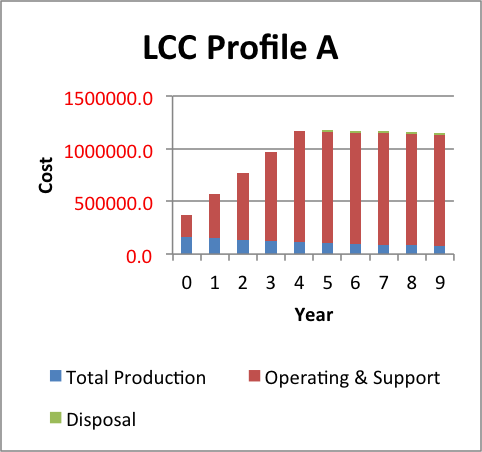
\includegraphics[scale=0.95]{images/LCCProfileA.png}
	\end{center}
	\caption{LCC Profile A}
	\label{fig:lccprofilea}
\end{figure}

\begin{figure}[h!tbp]
	\begin{center}
		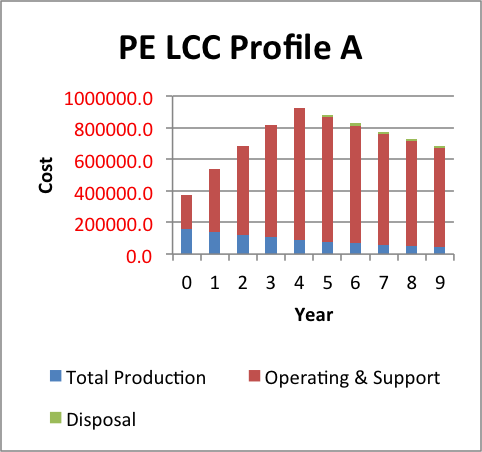
\includegraphics[scale=0.95]{images/PELCCProfileA.png}
	\end{center}
	\caption{PE LCC Profile A}
	\label{fig:pelccprofilea}
\end{figure}

\begin{figure}[h!tbp]
	\begin{center}
		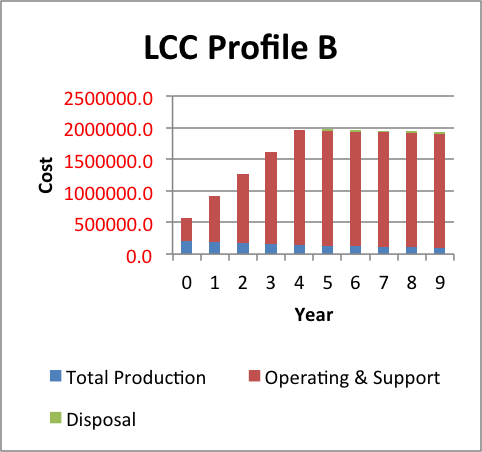
\includegraphics[scale=0.95]{images/LCCProfileB.png}
	\end{center}
	\caption{LCC Profile B}
	\label{fig:lccprofileb}
\end{figure}

\begin{figure}[h!tbp]
	\begin{center}
		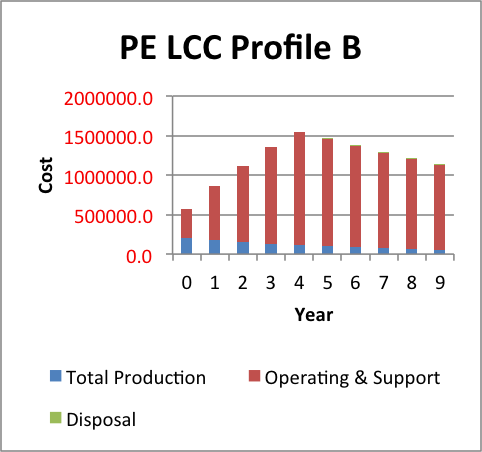
\includegraphics[scale=0.95]{images/PELCCProfileB.png}
	\end{center}
	\caption{PE LCC Profile B}
	\label{fig:pelccprofileb}
\end{figure}

\begin{figure}[h!tbp]
	\begin{center}
		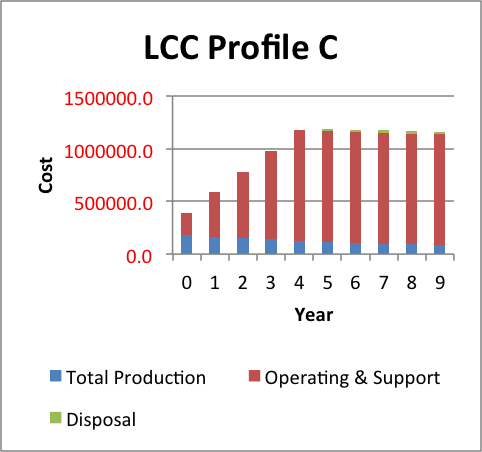
\includegraphics[scale=0.95]{images/LCCProfileC.png}
	\end{center}
	\caption{LCC Profile C}
	\label{fig:lccprofilec}
\end{figure}

\begin{figure}[h!tbp]
	\begin{center}
		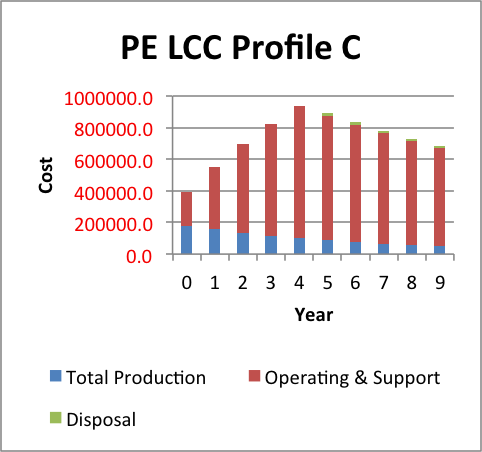
\includegraphics[scale=0.95]{images/PELCCProfileC.png}
	\end{center}
	\caption{PE LCC Profile C}
	\label{fig:pelccprofilec}
\end{figure}

\end{document}
